\chapter{Introduction}
{\color{red} write this intro bit!}

\section{Background to the study}
Some researchers turn bio-mimicry for insight and inspiration into the design of robots. One such example is the University of Cape Town (UCT) mechatronics laboratory's Rapid Acceleration and Manoeuvrability group, which studies cheetahs with the aim of reproducing their extraordinary manoeuvrability in two and four legged robots {\color{red} (cite)}. To understand the dynamics of cheetah movement, they require footage of animals as they start and stop a sprint. The cameras must be placed in pairs to achieve depth perception. {\color{red} (cite)}

The researchers currently place multiple static cameras, with each pair covering a different area, in order to continuously film an animal through a full sprint. An illustration of this can be seen in Figure~\ref{fig:multiple_gopro_pairs}. \\

% TODO: cite picture from change.org 'add cheetah emoji' petition?
\begin{figure}[h!]
  \centering
  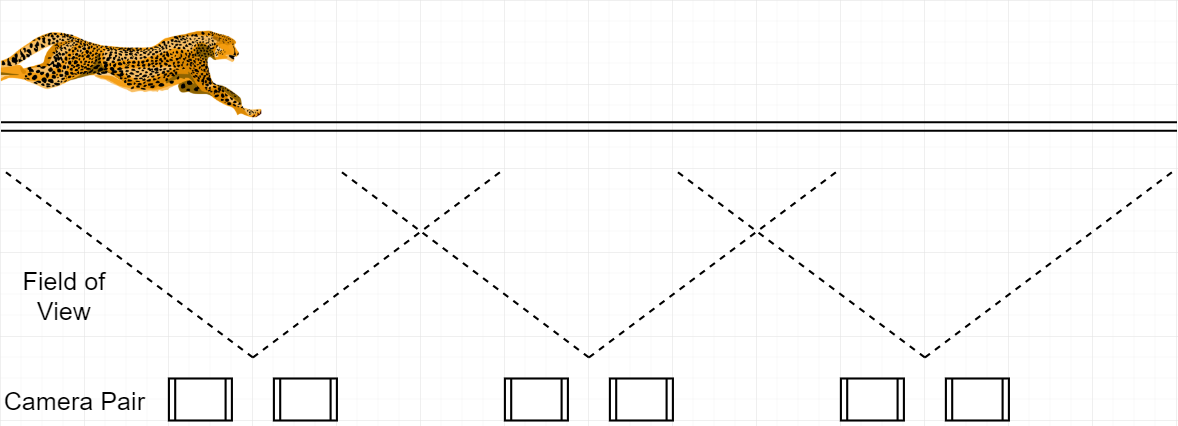
\includegraphics[width=\textwidth]{multiple_gopro_pairs}
  \caption{\label{fig:multiple_gopro_pairs} An illustration of the camera set up in a typical animal movement study.}
\end{figure}

Unfortunately, this setup is not without its disadvantages: having multiple cameras requires extra setup time, effort into synchronizing the footage, money spent on equipment and extra work in keeping all devices charged. To maximise the time spent recording a sprint, the cameras are usually set to wide-angle mode. This introduces distortion into the recordings. {\color{red} (cite)}

This resulted in the following question: what if the cameras could instead rotate to track the cheetah as it moves? This way only a single pair of cameras would be required. An illustration of this in two moments of time is shown in Figure~\ref{fig:single_gopro_pair}.

\begin{figure}[h!]
  \centering
  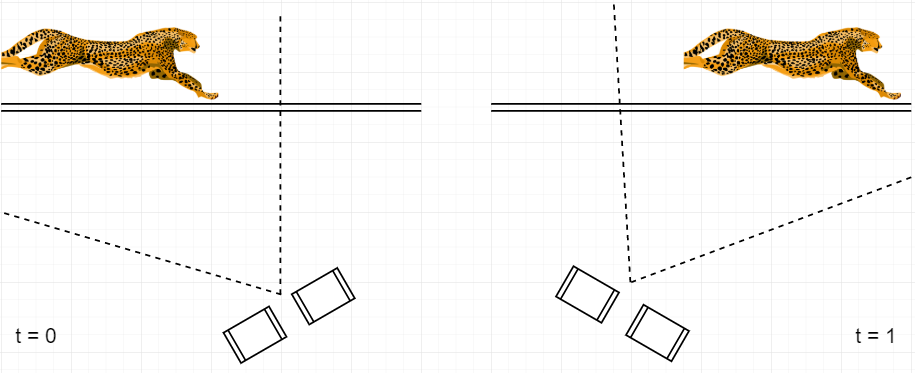
\includegraphics[width=\textwidth]{single_gopro_pair}
  \caption{\label{fig:single_gopro_pair} The proposed solution: a single pair of cameras tracking an animal as it moves.}
\end{figure}

After comparing existing object tracking technologies, it was decided that the only way to robustly track the cheetahs in this scenario would be to use a neural network. This decision is elaborated on in section \ref{sec:compare_cv_techniques} of this report. In short, the comparison showed that only machine learning techniques can accurately discriminate between a range of classes of objects. It , using affordable and accessible hardware (such as cameras) alone.

In order to not disturb the animal, it is desired to keep the tracked object free of any sensor equipment - for this reason, and for other elaborated in section {\color{red} xxx}, it was desired that a neural network would be used to identify and track the cheetah. {\color{red} stop here or keep going an properly introduce the idea of using computer vision, etc?} {\color{red} this should be the point where i mention that a Pi/low-power SBC was used for the study}

\section{Objectives of the study}
Based on the problems stated by the UCT researchers, the objective of the study is to design, build and test a system which can autonomously identify and track a fast-moving object using modern computer vision methods. A successful design would be able to rotate a pair of cameras to continuously aim at an object, track the object for longer, and not require the cameras to be set to distorting wide-angle modes.

Note that, while the ability to autonomously track an object has a wide range of applications {\color{red} (cite)}, it is useful to limit oneself to a particular need in order to produce quantifiable 'success or failure' metrics. Thus, this project and report are mainly about solving a specific issue, with the premise that the project can be used for other applications with minimal modification. Discussions on literature and other applications will treat the system as a general purpose object tracker.


\section{Other design requirements}
Additionally, the researchers specified that the object tracker should,

\begin{itemize}
	\item Not require a beacon, light or any other object to be placed on the object,
	\item Locate the object with high accuracy,
	\item Be able to differentiate between classes of objects, while treating different instances of the same class equally (in other words, locate \emph{any} cheetah regardless of its specific spot pattern),
	\item Have a low enough latency that the object can't escape the field of view of the cameras before a result is reached,
	\item Be mobile, which means not required access to a powerful stationary computer,
	\item Work robustly - this means locating the regardless of its orientation, lighting, specific shape, background, and so on - and finally,
	\item Be able to track any other object with minimal extra work or design required, should the focus of research be changed.
\end{itemize}


\section{Scope and limitations}
Due to the limited time and finances in an undergraduate thesis, the system was not tested on actual cheetahs during the course of the project. Instead, it was tested on humans in complex environments with the hope that this sufficiently mimics the scenario of tracking cheetahs (or any other fast-moving object, for that matter).

%However, the neural network will be retrained to be able to track cheetahs. This will be tested in simulation.

Finally, the study was limited to tracking only one object in the frame at a time. This is because it is not immediately obvious what should be done when more than one object is present in the frame.


\section{Plan of development}
A development schedule was devised to decide how much time could be allotted for each component of the final system. It was as follows,

\begin{enumerate}
\item Create a rough design for the system as a whole to understand which skills and components would be necessary.
\item Spend a month learning relevant new theory, mostly in the field of computer vision.
\item Set up the main computing platforms, installing relevant software and testing the camera module, over the course of a week.
\item Choose a neural network architecture and deploy it onto a neural accelerator stick.
\item Use two weeks to design and 3D print a camera gimbal, and procure the necessary controller and actuators.
\item At the same time, rewrite the gimbal controller communication standard in python to allow the raspberry pi to send and receive commands.
\item Model the expected movement of the tracked object, and then design and implement a Kalman Filter. Continuously update this based on preliminary results. 
\item Spend two weeks implementing a parallel process-based data pipeline which takes a photo on the Pi camera, pre-processess it, passes it through the neural accelerator, retrieves the results, passes the results into the Kalman Filter and then commands the gimbal motors to re-orient the camera appropriately. 
\item Test final the system over the course of a week, tweaking the design based on results.
\item Use the last three weeks to write a report which summarizes the entire project, based on small notes taken during the course of the project.
\end{enumerate}




\section{Other object tracking systems}
% possibilities: https://www.movidius.com/applications
There are a large number of applications for a system which can track objects in real time. Some include:

\begin{itemize}
\item A robot which can sense nearby humans and make sure to not hurt them, or decide on a course of action which depends on the type of object in front of it.
\item A small autonomous airplane which patrols the skies above a national park, and broadcasts the location of any potential poachers that it finds.
\item A camera system which automatically tracks a ball or the centroid of the position all players, helping to record sports games.
\end{itemize}

Object tracking systems have already been incorporated into existing commercial products, such as the "Maviv" drone from DJI, can autonomously track humans {\color{red} (cite)}. This allows people to launch the drone and have it autonomously follow them as they move around.

Another example is EyeCloud, a company that has developed a security system which covers a wider area than a single static camera could, and only sends an alert when it detects humans {\color{red} (cite)}. This stops false alarms when safe classes of objects, such as dogs, enter the field of view.




\section{Report outline}

The report begins with a review of the current literature surrounding object tracking. As the system combines a number of technologies, it also presents previous knowledge on all of the components which ultimately formed a part of final system.

Next, a more detailed description of the problem, plan of action, activities and project timeline are provided.

Following that are a few chapters which discuss the actual methodology used in the design and implementation of the tracking system. This is done with the aim that reproducing and extending the project can be done with minimal effort.

The results of testing the system are then shown.

Finally, the report ends off with conclusions on the project's success or failure, along with recommendations for future work.
